\documentclass[titlepage,usenames,a4,landscape,semhelv]{seminar}
\newcommand{\presenter}{Abram Hindle}
\newcommand{\conference}{}
\newcommand{\gettitle}{What's Hot and What's Not:\\Windowed Developer Topic Analysis}

\newcommand{\gettitleproper}{\gettitle}
\newcommand{\names}{Abram Hindle, Micheal W. Godfrey, Richard C. Holt}
\author{
\names \\ 
{\small Software Architecture Group }\\
\small David R. Cheriton School of Computer Science\\
\small University of Waterloo\\
\small Canada\\
ahindle@cs.uwaterloo.ca
}


\include{header}

\newcommand{\imageslide}[2]{
\newslide
\includegraphics[width=0.9\textwidth]{#2}
}

\newcommand{\figcaption}[1]{
\begin{center}
#1\\
\end{center}
}


\newcommand{\ig}[1]{\includegraphics{#1}}
%%%%%%%%%%%%%%%%%%%%%%%%%%%%%%%%%%%%%%%%%%%%%%%%%%%%%%%%%%%%%%%%%%%%%%%%%%%%%%%%
\begin{document}
\pagestyle{fancy} %bars..
\begin{slide}

\begin{center}
{\bf \LARGE \gettitleproper }

{\names } 

{\small Software Architecture Group }\\[-.5em]
{\small David R. Cheriton School of Computer Science}\\[-.5em]
{\small University of Waterloo}\\[-.5em]
{\small Canada}\\[-.5em]
{\small http://swag.uwaterloo.ca/}\\
\{ahindle,migod,holt\}@cs.uwaterloo.ca


\end{center}

=Figure 1
* Show a stream of of changes

=Introduction
* Stakeholders want to know what the focus of the last iteration was
* Evidence of work done at Retrospective meetings
* Difference between developer opinion and developer commits


=Dictionary
* Message - in this a CVS Commit
* Word Distribution - count of words occuring in a message
* Topic - a word distribution that is common amongst messages
* Trend - a topic that re-occurs


=Developer Trends
* Trends
** Continuous or repeating topics
** Occur over multiple time windows

=LDA
* Latent Dirichlet Allocation
* Like Latent Semantic Indexing (LSI)
* Like ICA/PCA
* Black box view:
** Input word distributions of messages, 
** Output topics consisting of a word distribution and related messages



=Topic Clustering 
* Need to track continuous topics across 
* Similarity between topics
* Clusters of the transitive closure of topics with X\% similarity
** Fill flood along similarity, make subsets of everyone who X\% similar to any of their neighbors, make that a cluster

%\newslide

\igonecap{transitiveclosure}{Clustering topics (black dots) by Transitive Closure based on similarity (arcs)}


=Topic Similarity
* Given 2 topics
** if their top 10 words 
*** share X words (7 or more)
****  they are similar




%\igbigslidecap{transitiveclosure}{Clustering topics (black dots) by Transitive Closure based on similarity (arcs)}

% \begin{center}
% 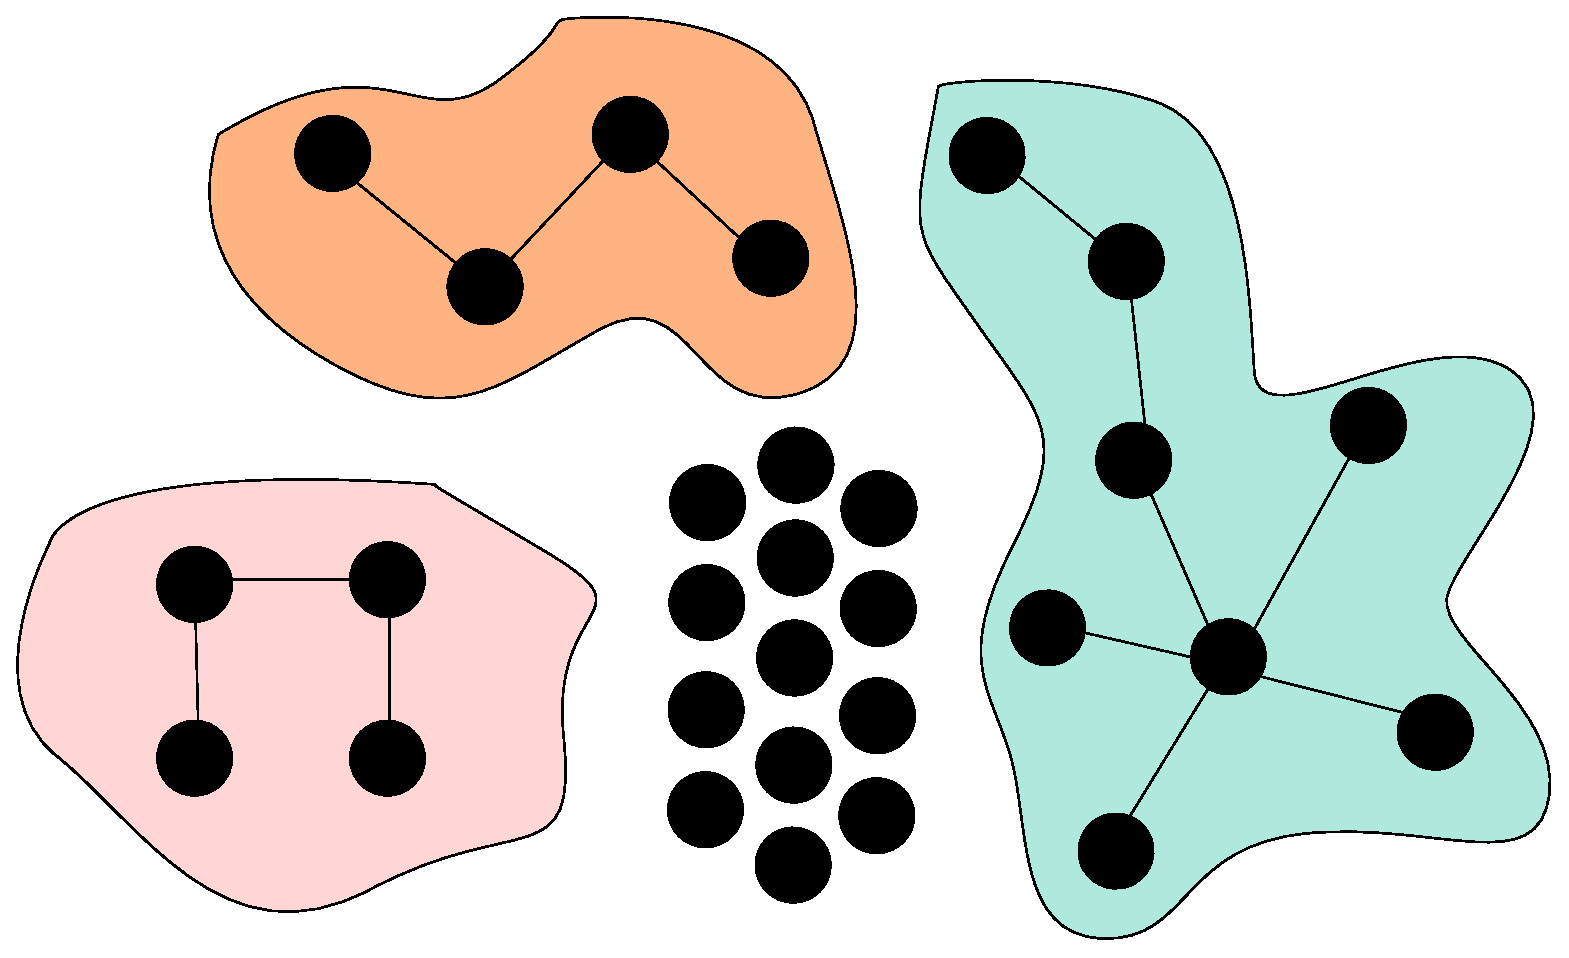
\includegraphics[width=\textwidth]{transitiveclosure}
% Clustering topics (black dots) by Transitive Closure based on similarity (arcs)
% \end{center}

%\igninetycap{transitiveclosure}{Clustering topics (black dots) by Transitive Closure based on similarity (arcs)}

\newslide

%\igbigcapb{commit-to-topics}{How commits are aggregated into Topics}
\begin{specquotei}
\begin{center}
\noindent
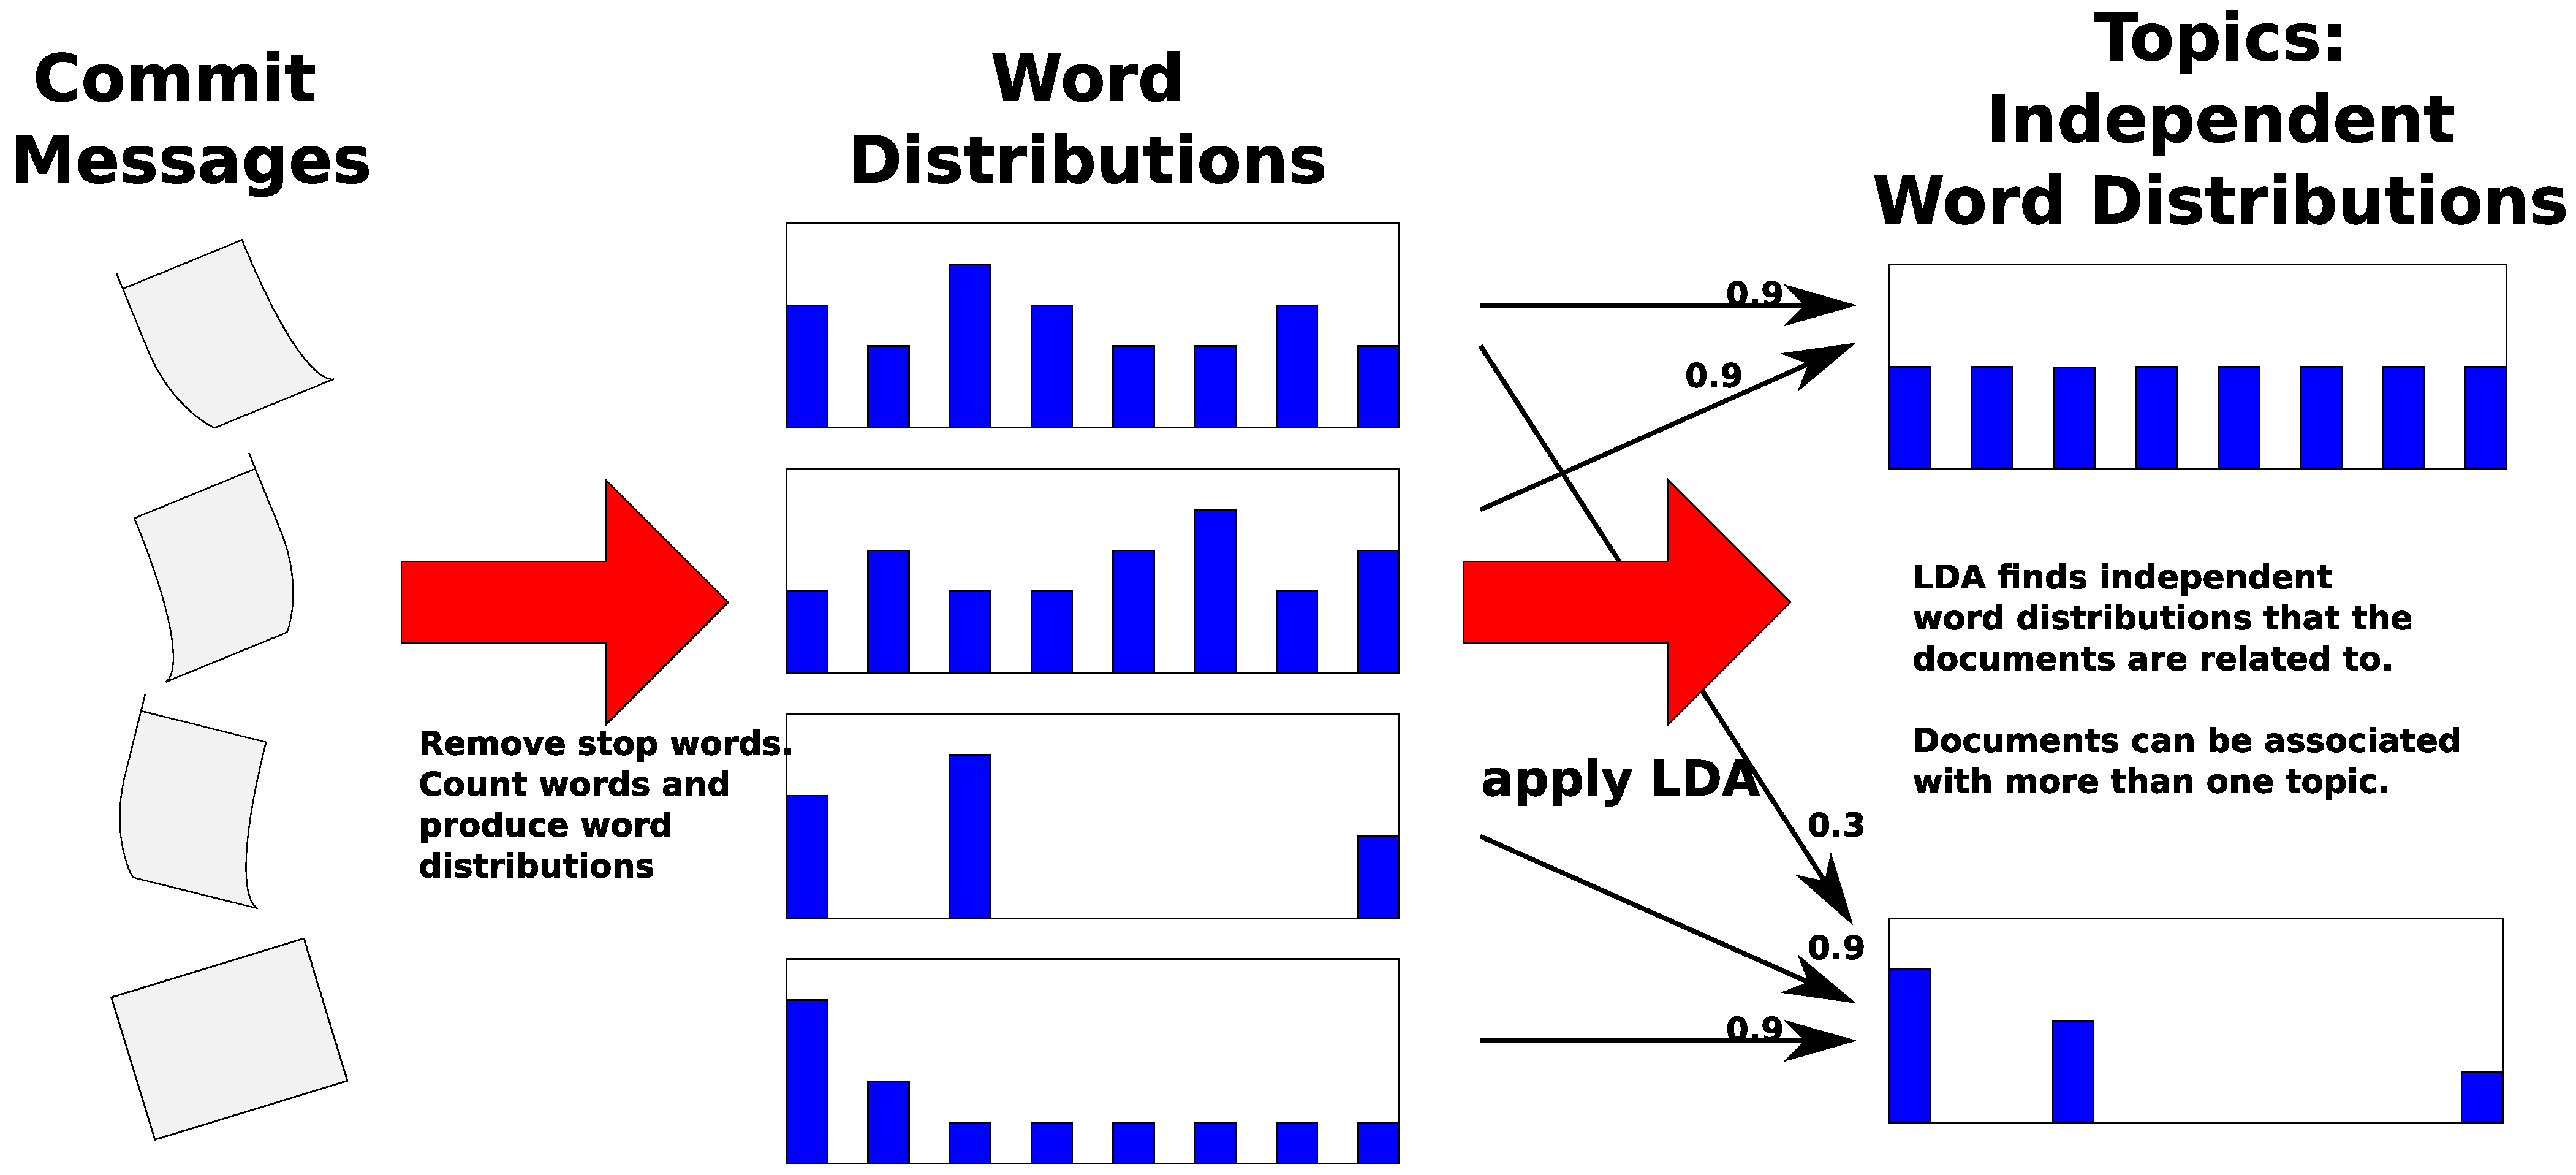
\includegraphics[width=1.25\textwidth]{commit-to-topics} \\
{How commits are aggregated into Topics}
\end{center}
\end{specquotei}

=Case Study: Portability
* MySQL 3.23 
** Discussions relating to portability
** Some topics trends (topics smeared across multiple months)


\newslide

%\begin{table*}
\begin{specquotef}
\centering
\begin{tabular}{|ccc|l|}

%\hline
%2000 &  Jul &  31 &    chmod \\
%2000 &  Sep &  29 &    fixes benchmark logging windows \\
%2000 &  Nov &  28 &    typo fix insert\_multi\_value \\
%2001 &  Jan &  27 &    fixes Innobase Cleanups auto-union \\
%2001 &  Mar &  28 &    2 topics bugfix, logging , TEMPORARY,  \\
\hline
2001 &  Jul &  26 &    update Allow TABLES LOCK [a] \\ 

2001 &  Aug &  25 &    tables row version [a] \\
\hline
%2001 &  Sep &  24 &    update checksum merge \\
%2001 &  Oct &  24 &    fixed fix \\
%2001 &  Dec &  23 &    HPUX SCO fix \\
\hline
2002 &  Feb &  21 &    net buffer length  max\_allowed\_packet [b] \\
2002 &  Mar &  23 &    small buf fix [b]  \\
%\hline
%2002 &  May &  22 &    [popular] fix SCO OSF1 table\_name \\
%2002 &  Nov &  18 &    HPUX11 compiler HP \\
\hline
\hline
2003 &  Feb &  16 &    Linux errno  [c] \\
2003 &  Mar &  18 &    alarm bookmark bug [c] \\
%\hline
%2003 &  Sep &  14 &    Auto logging merge windows distribution fix 64-bit 4.0 Cleanup \\
\hline
\end{tabular} \\
%\caption{Continuous blocks found while tracking topics associated with the word portability in MySQL 3.23}
{Continuous blocks found while tracking topics associated with the word portability in MySQL 3.23}
\label{tab:portability}
%\end{table*}
\end{specquotef}



% \begin{figure}
%   \centering
%   \includegraphics[width=1.5\textwidth]{lda}
%   \caption{Example of topics extracked from MySQL 3.23}
%   \label{fig:mysql323}
% \end{figure}

%\igbigslidecap{lda}{Example of topics extracted from MySQL 3.23}
%\igonecap{lda}{Example of topics extracted from MySQL 3.23}
%\igbigcapb{lda}{Example of topics extracted from MySQL 3.23}
%\igbigthirtycapb{lda}{Example of topics extracted from MySQL 3.23}

%\newslide

\igbigthirtyfivecapb{lda}{Example of topics extracted from MySQL 3.23. This is the kind of plot we eventually want to produce: named topics and topic trends}

%\newslide

=Case Study: MaxDB 7.500
* Autogenerated plots from MaxDB 7.500
* Multiple Presentations
** Condensed view
** Trend Histogram 
** Trend View
** Trend Timeline


\igbigcap{fixed-time-smear-plot-cropped}{Slice of Topics per Month for MaxDB 7.500}

%\newslide

\igonecap{fixed-time-smear-plot-scaled}{Entire View of Topics per Month for MaxDB 7.500}   

%\newslide

%\igninetycap{histogram-cropped}{}

%\newslide

\igHeigthyfivecap{histogram-cropped-scaled}{Top part of trend histogram, ordered by topic occurance}       

\newslide

\igonecap{class-smear-plot-crop-scaled}{Trend Time Line: Trends plotted over time of MaxDB 7.500}         

\newslide

%\igbigcapb{class-smear-plot-crop-scaled-zoomed}{Zoomed in view of the repeating topics plotted}
\begin{specquoteh}
\begin{center}
\includegraphics[width=1.25\textwidth]{class-smear-plot-crop-scaled-zoomed} \\
Zoomed in view of the trend time line
\end{center}
\end{specquoteh}

%\igbigcapb{class-smear-plot-crop-scaled-zoomed}{Zoomed in view of the repeating topics plotted}



=Observations
* Topics could be named
** Certain words indicate a focus on
*** Maintenance
*** Bug Fixing
*** Portability
*** Potential 'ilities

=Observations
* Powerlaw distribution of repeating topic counts
** Most occured once
** A few were repeated 
*** less than 10\% of topics reoccur

=Unfinished
* Total Topics versus Monthly Topics
* Clean up plots

=Future work
* Cluster Naming
* Associate trends with software taxonomies
** Extension, associate Trends or Topics with purpoes by using wordnet and Taxonomies of software quality as suggested by Ernst et al.
* Validation

=Conclusions
* Contributions
** Auto extract trends
*** Present trends
** Apply topic analysis on timewindows rather than the entire project




=
\end{slide}


\end{document}
